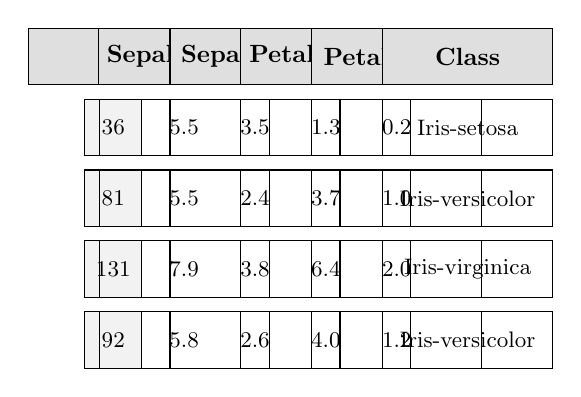
\begin{tikzpicture}[
    scale=0.9,
    transform shape,
    cell/.style={
        draw,
        minimum width=2.4cm,
        minimum height=0.8cm,
        align=center,
        font=\small
    },
    index/.style={
        cell,
        minimum width=0.8cm,
        fill=gray!10
    },
    header/.style={
        cell,
        fill=gray!25,
        font=\bfseries
    }
]

% =====================
% Encabezado
% =====================
\node[header] at (0,0) {};
\node[header] at (1,0) {Sepal length};
\node[header] at (2,0) {Sepal width};
\node[header] at (3,0) {Petal length};
\node[header] at (4,0) {Petal width};
\node[header] at (5,0) {Class};

% =====================
% Fila 36
% =====================
\node[index] at (0,-1) {36};
\node[cell]  at (1,-1) {5.5};
\node[cell]  at (2,-1) {3.5};
\node[cell]  at (3,-1) {1.3};
\node[cell]  at (4,-1) {0.2};
\node[cell]  at (5,-1) {Iris-setosa};

% =====================
% Fila 81
% =====================
\node[index] at (0,-2) {81};
\node[cell]  at (1,-2) {5.5};
\node[cell]  at (2,-2) {2.4};
\node[cell]  at (3,-2) {3.7};
\node[cell]  at (4,-2) {1.0};
\node[cell]  at (5,-2) {Iris-versicolor};

% =====================
% Fila 131
% =====================
\node[index] at (0,-3) {131};
\node[cell]  at (1,-3) {7.9};
\node[cell]  at (2,-3) {3.8};
\node[cell]  at (3,-3) {6.4};
\node[cell]  at (4,-3) {2.0};
\node[cell]  at (5,-3) {Iris-virginica};

% =====================
% Fila 92
% =====================
\node[index] at (0,-4) {92};
\node[cell]  at (1,-4) {5.8};
\node[cell]  at (2,-4) {2.6};
\node[cell]  at (3,-4) {4.0};
\node[cell]  at (4,-4) {1.2};
\node[cell]  at (5,-4) {Iris-versicolor};

\end{tikzpicture}
